\section{Раздел 6: ряды задачи}
1. Как 45 орехов разложить на 9 тарелок так, чтобы в каждой было разное количество орехов?\\
2. Как 55 орехов разложить на 10 тарелок так, чтобы в каждой было разное количество орехов?\\
3. Бревно нужно распилить на 6 частей. За сколько времени это можно сделать, если один распил занимает 1 мин 30 сек?\\
4. Бревно нужно распилить на 8 частей. За сколько времени это можно сделать, если один распил занимает 1 мин 30 сек?\\
5. Как 55 грибов разложить на 9 тарелок так, чтобы в каждой тарелке было разное количество грибов?\\
6. Как 65 орехов разложить на 10 тарелок так, чтобы в каждой тарелке было разное количество орехов?\\
7. Дядя Фёдор, кот Матроскин, Шарик и почтальон Печкин сидят на скамейке. Если Шарик, сидящий справа от всех, сядет между дядей Фёдором и котом, то кот будет крайним слева. В каком порядке они сидят?\\
8. Бабушка, папа, мама и девочка сидят на скамейке. Если мама, сидящая слева от всех, сядет между бабушкой и папой, то папа будет крайним справа. В каком порядке они сидят?\\
9. Сколько натуральных чисел расположено между числами 17 и 43?\\
10. Сколько натуральных чисел расположено между числами 19 и 53?\\
11. На прямой отмечено 200 точек так, что расстояние между любыми соседними точками равно 2 см. Чему равно расстояние между крайними точками?\\
12. На прямой отмечено 180 точек так, что расстояние между любыми соседними точками равно 5 см. Чему равно расстояние между крайними точками?\\
13. Учебный год у Незнайки --- 239 учебных дней. Но не сразу этот неряха сообразил приобрести форменный галстук. И носил его только с 39-го дня до 239-го. Сколько дней Незнайка щеголял в форменном галстуке?\\
14. Незнайка обнаружил в школьной библиотеке 239 книг по математике и забрал себе те, что стояли с краю: от 200-й до 239-й. Сколько книг пришлось ему тащить обратно?\\
15. Будем называть число {\bf утренним,} если в его записи есть хотя бы одна чётная цифра. Перед вами ряд чисел: 1, 791, 1235, 3124, 6876, 9753, 10005, 99513, 217860, 77759, 1000000.\\
а) Сколько среди них утренних чисел?\\
б) Какова сумма утренних чисел в этом ряду?\\
16. Будем называть число {\bf вечерним,} если в его записи есть хотя бы одна чётная цифра. Перед вами ряд чисел: 2, 101, 2398, 5319, 7039, 7735, 9899, 80800, 13579, 997579.\\
а) Сколько среди них вечерних чисел?\\
б) Какова сумма вечерних чисел в этом ряду?\\
17. Сколько чисел от 1 до 900 не делятся на 30?\\
18. Сколько чисел от 1 до 750 не делятся на 25?\\
19. В течение учебного года каждый день (включая выходные и праздники), с 1 сентября по 30 апреля Вася съедает ровно один йогурт. Сколько йогуртов он съел за 4 года обучения в начальной школе, поступив в школу в 2009 году?\\
20. В течение учебного года каждый день (включая выходные и праздники), с 1 октября по 31 мая Вася съедает ровно один банан. Сколько бананов он съел за 4 года обучения в начальной школе, поступив в школу в 2009 году?\\
21. Магазин мебели придумывает названия для своих товаров, которые должны состоять из нескольких букв подряд. Название признаётся {\it красивым,} если в нём количество букв {\bf А} и количество букв {\bf Б} отличается не более чем на одну. Перед вами ряд названий: БАБА, БРАМСОНКАРЛСЁ, НЯНЯ, ХЕНСВИКСТУВАСУНДВИК, БАНЯ, ПАНОРАМА, ОБАМА, АЛЬБРУОВЕРБУ, АТТЕСТЬТЪОСТЕРУП, СУНДЭККЕНУТНЭСФУНБУ, АБРАКАДАБРА. Сколько среди них красивых?\\
22. Магазин мебели придумывает названия для своих товаров, которые должны состоять из нескольких букв подряд. Название признаётся {\it красивым,} если в нём количество букв {\bf К} и количество букв {\bf У} отличается не более чем на одну. Перед вами ряд названий: КУКУ, РОДЬДЪСТОРПОВЕРУД, КАЮК, ПСАКИ, СУНДЭККЕНУТНЭСФУНБУ, КУСАЧКИ, СЭРОТОСТЕРО, БРУКЁКЛАССЕН, КУМУШКА, ХЕНСВИКСТУВАСУНДВИК. Сколько среди них красивых?\\
23. Будем называть число {\bf почётным,} если в его записи не более трёх чётных цифр (например, в числе 2239 две чётные цифры). Сколько почётных чисел в данном ряду: 2239, 100, 31337779, 324577711189, 31415926, 300201, 1000, 2390, 2468, 12357866, 111?\\
24. Будем называть число {\bf зачётным,} если в его записи не более трёх чётных цифр (например, в числе 2239 две чётные цифры). Сколько зачётных чисел в данном ряду: 2239, 1100, 77313379, 70010, 2390, 6824, 78661235, 777, 771113245789, 2718281828, 201300?\\
25. Сколько чисел от 159 до 241 содержат в своей записи хотя бы одну тройку?\\
26. Сколько чисел от 239 до 321 содержат в своей записи хотя бы одну четвёрку?\\
27. Число называется {\it превосходным,} если в его записи нет повторяющихся цифр и среди цифр есть ровно 2 чётных. Какие из следующих чисел превосходны? 1234, 2053, 25958, 1894725, 4703519, 8956713, 9753010. В ответ запишите их количество.\\
28. Число называется {\it превосходным,} если в его записи нет повторяющихся цифр и среди цифр есть ровно 2 чётных. Какие из следующих чисел превосходны? 2345, 1027, 13243, 27018359, 2454314, 8956703, 13247, 305709. В ответ запишите их количество.\\
29. Сколько чётных чисел от 239 до 1001?\\
30. Сколько чётных чисел от 501 до 1239?\\
31. В поезде метро 8 вагонов, в каждом из которых 4 двери для пассажиров. При поездке с <<Девяткино>> на <<Чернышевскую>>, чтобы сразу выйти на эскалатор, нужно выходить из третьей двери третьего вагона, если считать с конца. Какой дверью какого вагона эта дверь будет, если считать от начала?\\
32. В поезде метро 8 вагонов, в каждом из которых 4 двери для пассажиров. При поездке с <<Автово>> на <<Чернышевскую>>, чтобы сразу выйти на эскалатор, нужно выходить из второй двери четвёртого вагона, если считать от начала. Какой дверью какого вагона эта дверь будет, если считать с конца?\\
33. Илья заказал в ресторане 2 чизбургера, 3 ролла и 6 порций картошки. Официант перепутал заказ и принёс ему 2 порции картошки, 3 чизбургера и 6 роллов. При этом стоимость заказа осталась прежней. Расположите чизбургер, ролл и картошку в порядке возрастания их цен, если известно, что чизбургер дороже ролла.\\
34. Серёжа заказал в кафе 3 хачапури, 4 бифштекса и 6 порций картошки. Официант перепутал заказ и принёс ему 3 порции картошки, 4 хачапури и 6 бифштексов. При этом стоимость заказа осталась прежней. Расположите хачапури, бифштекс и картошку в порядке возрастания их цены, если известно, что хачапури дороже бифштекса.\\
35. Слово называется {\it хорошим,} если количества букв <<р>> и <<а>> в этом слове отличаются не более чем на два (например, слова {\it рак, барак, рубрификатор} --- хорошие). К хорошему слову приписали <<рурирор>> и получили хорошее слово с 4 буквами <<а>>. Сколько в исходном слове букв <<р>>?\\
36. Слово называется {\it хорошим,} если количества букв <<р>> и <<а>> в этом слове отличаются не более чем на два (например, слова {\it рак, барак, рубрификатор} --- хорошие). К хорошему слову приписали <<абракакадабра>> и получили хорошее слово с 7 буквами <<р>>. Сколько в исходном слове букв <<а>>?\\
37. Сколько чисел от 459 до 671 содержат в записи одновременно цифры 5 и 6?\\
38. Сколько чисел от 239 до 457 содержат в записи одновременно цифры 3 и 4?\\
39. Анна, Божена, Вера, Галина, Дарья и Евгения соревновались в решении задач. Анна обогнала Галину и ещё двоих. Божена и Евгения вместе решили столько же задач, сколько Вера и Дарья вместе. Вера решила меньше задач, чем Галина, но больше, чем Божена. Кто какое место занял? Запишите первые буквы их имён в порядке убывания числа решённых задач (например, АГДБЕВ).\\
40. Антон, Борис, Василий, Георгий, Дмитрий и Евгений соревновались в решении задач. Антон пропустил вперёд Георгия и ещё двоих. Борис и Дмитрий вместе решили задач столько же, сколько Василий и Евгений вместе. Дмитрий решил задач больше, чем Георгий, но меньше, чем Василий. Кто какое место занял? Запишите первые буквы их имён в порядке убывания числа решённых задач (например, АГДБЕВ).\\
41. Продолжите последовательность 1; 15; 45; 59; 177; ... ещё двумя числами.\\
42. Продолжите последовательность 3; 19; 57; 73; 219; ... ещё двумя числами.\\
43. Ученики четвёртого класса после уроков пошли в парк. Учительница попросила их построиться четвёрками. Олеся, Таня, Аня и Алиса заметили, что их четвёрка пятая спереди и четвёртая сзади. Сколько учеников пошли в парк?\\
44. Антон нашёл старую книгу, в которой не хватало нескольких страниц. Последняя страница перед потерянной частью имеет номер 12, а первая после неё --- 39. Сколько листов выпало из книги?\\
45. Кабины колеса обозрения в парке аттракционов расположены через равные промежутки и пронумерованы подряд, начиная с 1. Когда в нижней точке находится кабина номер 4, в самой верхней точке находится кабина номер 19. Сколько всего кабин у колеса обозрения?\\
46. Спицы на колесе кареты расположены через равные промежутки и пронумерованы подряд, начиная с 1. Когда в нижней точке находится спица номер 11, в самой верхней точке находится спица номер 26. Сколько всего спиц у колеса кареты?\\
47. Порядок чисел в последовательности определён закономерностью. Продолжите последовательность ещё двумя числами: 3; 4; 9; 16; 15; 36; 21; ...\\
48. Порядок чисел в последовательности определён закономерностью. Продолжите последовательность ещё двумя числами: 1; 14; 9; 28; 25; 42; 49; ...\\
49. Продолжите последовательность чисел ещё тремя числами: 2; 6; 7; 21; 22; ...\\
50. Продолжите последовательность чисел ещё тремя числами: 0; 0; 0; 1; 3; 1; 2; 6; 4; 3; 9; 9; 4; 12; 16; ...\\
51. Среди чисел 1234554, 2345645, 3464574, 5767897, 4357563 найдите все такие, в которых не более трёх чётных цифр и не менее двух цифр, делящихся на 3.\\
52. Сколько чисел, больших 533 и не превосходящих 1001, делятся на 7?\\
53. Садовник посадил в ряд десять кустов сирени. Затем между каждыми двумя кустами сирени он посадил по кусту жасмина. А на следующий год между каждыми двумя кустами он посадил по кусту шиповника. Сколько кустов шиповника посадил садовник, если зимой не замёрз ни один куст?\\
54. Вдоль длинной пустой дороги припарковалось 12 <<Мерседесов>>. Через час между каждыми двумя <<Мерседесами>> припарковалось по <<Фольцвагену>>. А ещё через час приехали велосипедисты и поставили по велосипеду между каждыми двумя машинами. Сколько поставлено велосипедов?\\
55. Если выписать подряд все числа от 1 до 299 включительно, то сколько всего цифр будет выписано?\\
56. Гном Торин положил в ряд несколько золотых монет. Гном Балин положил в ряду между каждыми двумя соседними золотыми монетами по две серебряные монеты. Затем гном Буфор положил между каждыми двумя соседними монетами по одной медной монете. Всего получилось 25 монет. Сколько среди них было золотых монет?\\
57. На полоске бумаги отмечены вертикальные линии красного, жёлтого и зелёного цвета. Если разрезать полоску по красным линиям, то получится 7 кусков, если по жёлтым --- 6 кусков, а если по зелёным --- 13 кусков. Сколько кусков получится, если полоску разрезать по линиям красного и зелёного цвета?\\
58. В субботу бобры распилили одно бревно. За день они сделали 10 распилов. Сколько получилось чурбачков?\\
59. В воскресенье Бобры поставили перед собой задачу: разрезать одно бревно на 12 частей. Сколько распилов им нужно сделать?\\
60. В понедельник Бобры распилили несколько брёвен. За день они сделали 10 распилов и получили 16 чурбачков. Сколько брёвен они распилили?\\
61. Во вторник на лесопилке было сделано 98 распилов и получено 113 чурбачков. Сколько брёвен распилили Бобры во вторник?\\
62. В среду Бобры пилили одно бревно длиной двадцать пять метров на куски длиной 1 дм каждый. Распиловка бревна поперёк занимает 3 минуты. За какое время Бобры распилили всё бревно?\\
63. В четверг знакомые Зайцы привезли Бобрам 60 трёхметровых брёвен. Их нужно было распилить на куски по 5 дм. Сколько распилов пришлось для этого сделать?\\
64. В пятницу приехали Суслики и сказали, что для строительство дома им необходимо купить 13 чурбачков по 2 метра. У Бобров на лесопилке можно купить длинные брёвна и распилить их. Прочитайте условия работы лесопилки и помогите Сусликам сделать наиболее выгодную покупку. Сколько рублей заплатят Суслики-строители Бобрам-пилителям?
\begin{figure}[h]
\center{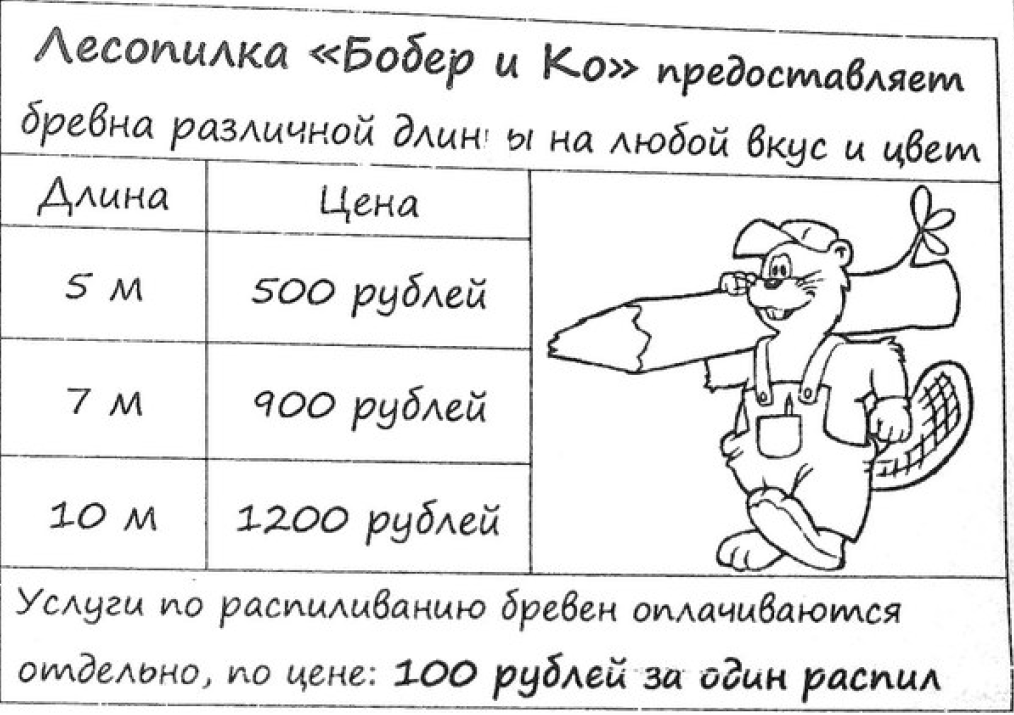
\includegraphics[scale=0.35]{1.png}}
\end{figure}\\
65. Вдоль шоссе стоят три дерева: береза, тополь, дуб. Расстояние между березой и тополем равно 23 м, а между тополем и дубом 47 м. Чему равно расстояние между березой и дубом?\\
66. Вдоль беговой дорожки расставлено 25 флажков на одинаковом расстоянии друг от друга. Вася стартует у первого флажка и бежит с постоянной скоростью. Через 20 секунд он оказывается у 5 флажка. Через какое время Вася добежит до 25 флажка?\\
67. Во сколько раз лестница на 7 этаж дома длиннее, чем лестница на 3 этаж этого же дома?\\
68. В одном ряду 8 камешков на расстоянии 2 см один от другого. В другом --- 15 камешков на расстоянии 1 см один от другого. Какой ряд длиннее?\\
69. Сколько чисел между 485 и  1234?\\
70. Этаж Сони 6 сверху в 25 этажном доме. На каком этаже живет Соня?\\
71. Гарри и Гермиона резали батон волшебной икательной колбасы. Они сделали 5 разрезов. Сколько получилось кусков колбасы?\\
72. Теперь они взяли батон хихикательной колбасы, сделали несколько разрезов и получили 10 кусков. Сколько разрезов они сделали?\\
73. На сей раз наши герои взяли несколько батонов щекотательной колбасы, сделали 8 разрезов и получили 13 кусков. Сколько батонов они взяли?\\
74. Лифт поднимается с первого этажа на третий за 6 секунд. За какое время он поднимется с первого этажа на девятый?\\
75. 12-метровую колбасу распилили на 3-метровые куски за 12 минут. А за сколько времени 12-метровую колбасу можно распилить на 1-метровые куски?\\
76. На каждой перемене Рон съедает по конфете. За неделю (с понедельника по субботу) было 30 уроков. Сколько всего конфет съел Рон?\\
77. Сколько нечётных чисел заключено между 300 и 700?\\
78. Из книги выпал кусок, первая страница которого имеет номер 439, а номер последней записывается теми же цифрами в каком-то другом порядке. Сколько страниц в выпавшем куске?\\
79. Маша испекла на Новый год три торта, для чего ей понадобилось в сумме десять коржей. Между каждыми двумя соседними коржами был намазан сливочный или шоколадный крем. Слоёв сливочного крема было пять. Сколько было слоёв шоколадного крема?\\
80. На глобусе провели 10 меридианов и 11 параллелей. Сколько кусков получилось? (Меридиан --- это дуга от полюса до полюса, параллель --– полный круг.)\\
81. Разрезали листочек на 5 частей, а одну из них --- ещё на 5 частей. Сколько частей получилось?\\
82. На полоске бумаги отмечены вертикальные линии синего, жёлтого и красного цвета. Если разрезать полоску по синим линиям, то получится 5 кусков, если по жёлтым --- 9 кусков, а если по красным --- 11 кусков. Сколько кусков получится, если разрезать полоску по линиям жёлтого и красного цвета?\\
83. Лист бумаги разрезали на три части, затем некоторые из полученных частей также разрезали на 3 части каждую, и так проделали несколько раз. Может ли при подсчёте количества всех частей получиться число 2018, и почему?\\
84. Герда положила в один ряд красные фишки. Затем Кай положил между двумя соседними красными фишками по одной синей. Затем Принц положил между каждыми двумя соседними фишками по две зелёные фишки. Всего получилось 19 фишек. Сколько красных фишек положила Герда?\\
85. Во сколько раз лестница на 4 этаж в школе длиннее лестницы на 2 этаж?\\
86. На каждом километре между городами Лево и Право стоит столб, на котором указано расстояние до обоих городов. Паша посчитал только столбы на которых есть цифра три. Сколько у него получилось столбов, если расстояние между городами 20 км?\\
87. На каждом километре между городами Лево и Право стоит столб, на котором указано расстояние до обоих городов. Паша посчитал только столбы на которых есть цифра пять. Сколько у него получилось столбов, если расстояние между городами 29 км?\\
88. Сколько натуральных чисел от 10 до 110 делится на 2?\\
89. Сколько натуральных чисел от 30 до 330 делится на 3?\\
90. а) Сколько чисел, больших 59 и меньших 1001, делятся на 7?\\
б) Сколько чисел, больших 59 и меньших 1002, делятся на 7?\\
91. а) Сколько чисел, больших 59 и меньших 2002, делятся на 13?\\
б) Сколько чисел, больших 60 и меньших 2003, делятся на 13?\\
92. 29 орехов разложили на несколько тарелок так, что на каждой тарелке хотя бы один орех и на любых двух тарелках разное количество орехов. Какое наибольшее число тарелок могло быть?\\
93. 37 орехов разложили на несколько тарелок так, что на каждой тарелке хотя бы один орех и на любых двух тарелках разное количество орехов. Какое наибольшее число тарелок могло быть?\\
94. Сколько чисел от 1239 до 2200 содержат в своей записи единицу?\\
95. Сколько чисел от 2239 до 3300 содержат двойку в своей записи?\\
96. Интервал между двумя последовательными поездами одинаков и составляет целое число минут. Марк ровно 60 минут смотрел на поезда и насчитал 8 проехавших мимо поездов. Каким может быть интервал движения?\\
97. Интервал между двумя последовательными поездами одинаков и составляет целое число минут. Марк ровно 90 минут смотрел на поезда и насчитал 12 проехавших мимо поездов. Каким может быть интервал движения?\\
98. Бобры Боб и Роб нашли очень длинное бревно для своей плотины. Боб сделал 15 распилов, а Роб распилил каждое получившееся у Боба брёвнышко на 3 части. Сколько в итоге получилось брёвнышек у бобров?\\
99. Сколько существует пятизначных чисел, делящихся на 15?\\
100. Сколько существует пятизначных чисел, делящихся на 21?\\
101. Будем называть число {\it весёлым,} если любые две его соседние цифры имеют разную чётность. Найдите сумму всех весёлых чисел среди данных: 12, 10, 2020206, 123458, 1001.\\
102. Будем называть число {\it грустным,} если любые две его соседние цифры имеют разную чётность. Найдите сумму всех грустных чисел среди данных: 21, 101, 6060602, 123458, 1001.\\
103. В последовательности 3, 4, 7, 1, 8, 9, 7 ... каждая цифра равна последней цифре суммы двух предыдущих цифр. Как видно, на 5-м месте стоит цифра 8. А какая цифра стоит на 2022-м месте?\\
104. В последовательности 9, 2, 1, 3, 4, 7, 1 ... каждая цифра равна последней цифре суммы двух предыдущих цифр. Как видно, на 5-м месте стоит цифра 4. А какая цифра стоит на 2022-м месте?\\
105. Когда Винни-Пух пришёл к Кролику, чтобы немножечко подкрепиться, он заметил, что в кладовой Кролика выше полки с самым вкусным мёдом и ниже неё одинаковое количество полок. Сначала он попробовал варенье, которое стояло тремя полками выше мёда, оттуда спустился на 7 полок вниз, так как там было сгущённое молоко. Так он оказался на 4 полке. Сколько полок в кладовой Кролика?\\
106. Когда кот Матроскин приехал в городскую квартиру Дяди Фёдора, он заметил, что выше этажа, где живёт Дядя Фёдор и ниже его одинаковое количество этажей. Сначала Матроскин случайно поднялся на 4 этажа выше этажа Дяди Фёдора, а потом спустился на 8 этажей вниз, так как забыл там на подоконнике бутерброд. Так он оказался на пятом этаже. Сколько всего этажей в доме, где живёт Дядя Фёдор?\\
107. Олег поставил в тетради точки по прямой линии так, что расстояние между соседними точками равно 3 см. Сколько точек поставил Олег, если расстояние между крайними равно 12 см?\\
108. Аня выше Нади, но ниже Кати. Инна выше Олеси, но ниже Ани. Кто из девочек самая высокая?\\
109. Будем называть число {\it однообразным,} если какие-то две его соседние цифры имеют одинаковую чётность. Найдите сумму всех однообразных чисел среди данных: 101010, 104060, 694936, 1003, 143256.\\
110. Будем называть число {\it однообразным,} если какие-то две его соседние цифры имеют одинаковую чётность. Найдите сумму всех однообразных чисел среди данных: 909090, 504020, 3001, 392978, 652341.\\
111. Сколько существует нечётных чисел, больших 239, но меньших 2339?\\
112. Сколько существует нечётных чисел, больших 239, но меньших 2139?\\
113. Для приготовления бутербродов Антон резал очень длинный батон. Сначала он сделал 11 разрезов, а потом каждый получившийся кусок разрезал ещё на 5 частей. Сколько всего кусков батона получилось?\\
114. Для приготовления бутербродов Алиса резала очень длинный батон. Сначала она сделала 4 разреза, а потом каждый получившийся кусок разрезала ещё на 14 частей. Сколько всего кусков батона получилось?\\
115. 2024 --- год дракона. Черепаха Джонатан родился в 1856 году и жив до сих пор. Сколько раз Джонатан застал год дракона? Год дракона наступает каждые 12 лет.\\
116. 2024 --- год дракона. Черепаха Джонатан родился в 1832 году и жив до сих пор. Сколько раз Джонатан застал год дракона? Год дракона наступает каждые 12 лет.\\
117. Сколько существует нечётных чисел, больших 239 и меньших 777?\\
118. Сколько существует нечётных чисел, больших 329 и меньших 777?\\
119. Трёхзначное число называется {\it красивым,} если его первая цифра чётная, последняя нечётная, а сумма всех трёх цифр равна 7. Сколько красивых чисел?\\
120. Трёхзначное число называется {\it красивым,} если его первая цифра чётная, последняя нечётная, а сумма всех трёх цифр равна 8. Сколько красивых чисел?

ewpage
